% this file is called up by thesis.tex
% content in this file will be fed into the main document



%: ----------------------- name of chapter  -------------------------
\chapter{Results} % top level followed by section, subsection

\ifpdf
    \graphicspath{{5_Results/figures/PNG/}{5_Results/figures/PDF/}{5_Results/figures/}}
\else
    \graphicspath{{5_Results/figures/EPS/}{5_Results/figures/}}
\fi

This chapter consists of discussions about the various results and performance metrics gathered over the course of training and testing the models. First, further training metrics are discussed and then the results from testing are considered.

\section{Training Loss}

\subsection{Model variation 1: SD Locked}

This was the best performing model out of the two with stark differences in the quality of generated images being observed even at the training phase. The Figures \ref{fig:mod1-train-loss-epoch} and \ref{fig:mod1-train-loss-epoch-smooth} represent the same loss with loss value plotted against number of epochs. From the first graph we can see that the loss has been very erratic and it unable to get to a convergence point. In fact, at around 20k steps ($\approx 20  epochs$), the epoch loss has managed to reach the lowest loss of 0.1763 while the last epoch i.e., 50 ended the training with the second lowest of 0.1778. The immediate realisation is that learning rate would need to be lowered.
\begin{figure}[h]
    \centering
    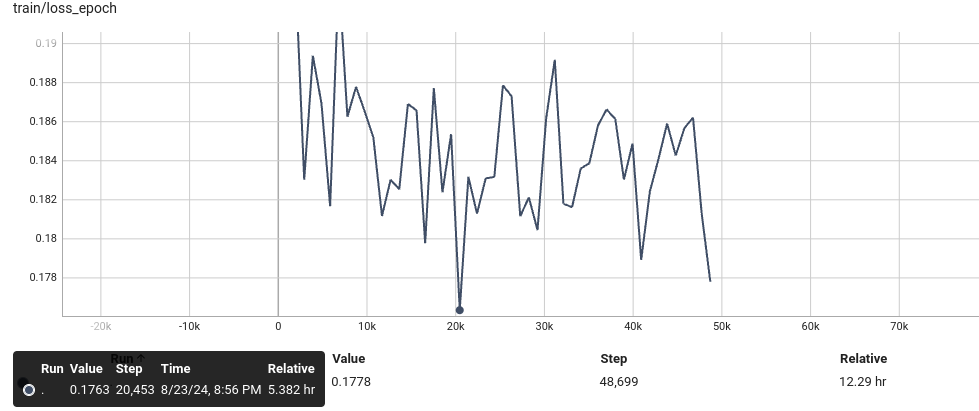
\includegraphics[width=1\linewidth]{5_Results/figures/var1-train-epoch-loss.png}
    \caption{Model 1: Train loss/epoch}
    \label{fig:mod1-train-loss-epoch}
\end{figure}
But when the smoothed curve is observed, there is an overall down slope to the learning which suggests that the training is in general moving in a positive direction but perhaps it would yield better results if the number of epochs were to be increased and training continued for a longer period of time. In fact, 50 epochs is not a high number at all when most such training projects train for epochs in the range of thousands. There is also an interesting note observed by the author \parencite[Figure 4, p. 5]{Zhang2023AddingModels} where the phenomenon of sudden convergence is observed after enough training steps. It should also be noted that ControlNets are mainly used with adding image masks such as depth, edge, segmentation maps as their control input for training which would contain way lesser spatial and structural data and more rigidity to the outcomes. With our use case being two different staining domains, these variations in performance is to be expected. 
\begin{figure}[h]
    \centering
    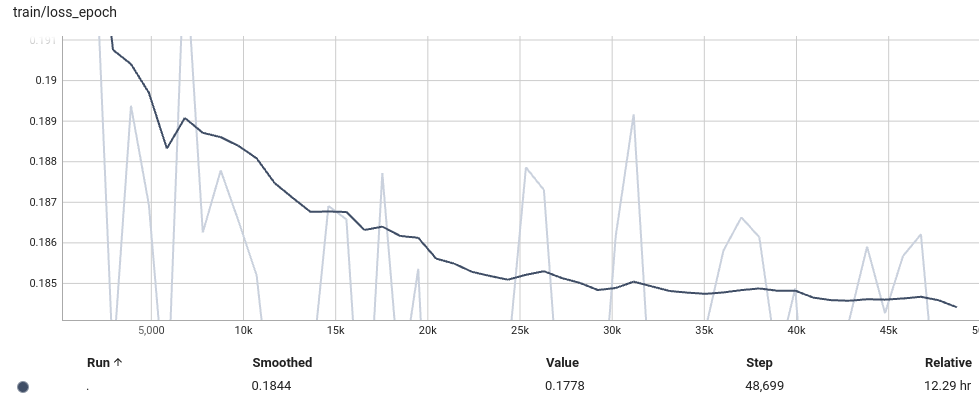
\includegraphics[width=1\linewidth]{5_Results/figures/model-1-train-loss-epoch-smooth.png}
    \caption{Model 1: Train loss/epoch with smoothing=0.9}
    \label{fig:mod1-train-loss-epoch-smooth}
\end{figure}

The four Figures \ref{fig:train-log-source-e20-s900}, \ref{fig:train-log-target-e20-s900}, \ref{fig:train-log-sample-e20-s900} and \ref{fig:train-log-prompt-e20-s900} is a training render sample that corresponds to the $900^{th}$ step in epoch 20 of training which is where the least loss was observed. This too has good structural and intensity mapping in the generated images. The colouring on the membranes of the cells and the patterns formed are very much comparable when performing a the simple eye test.
\begin{figure}[h]
    \centering
    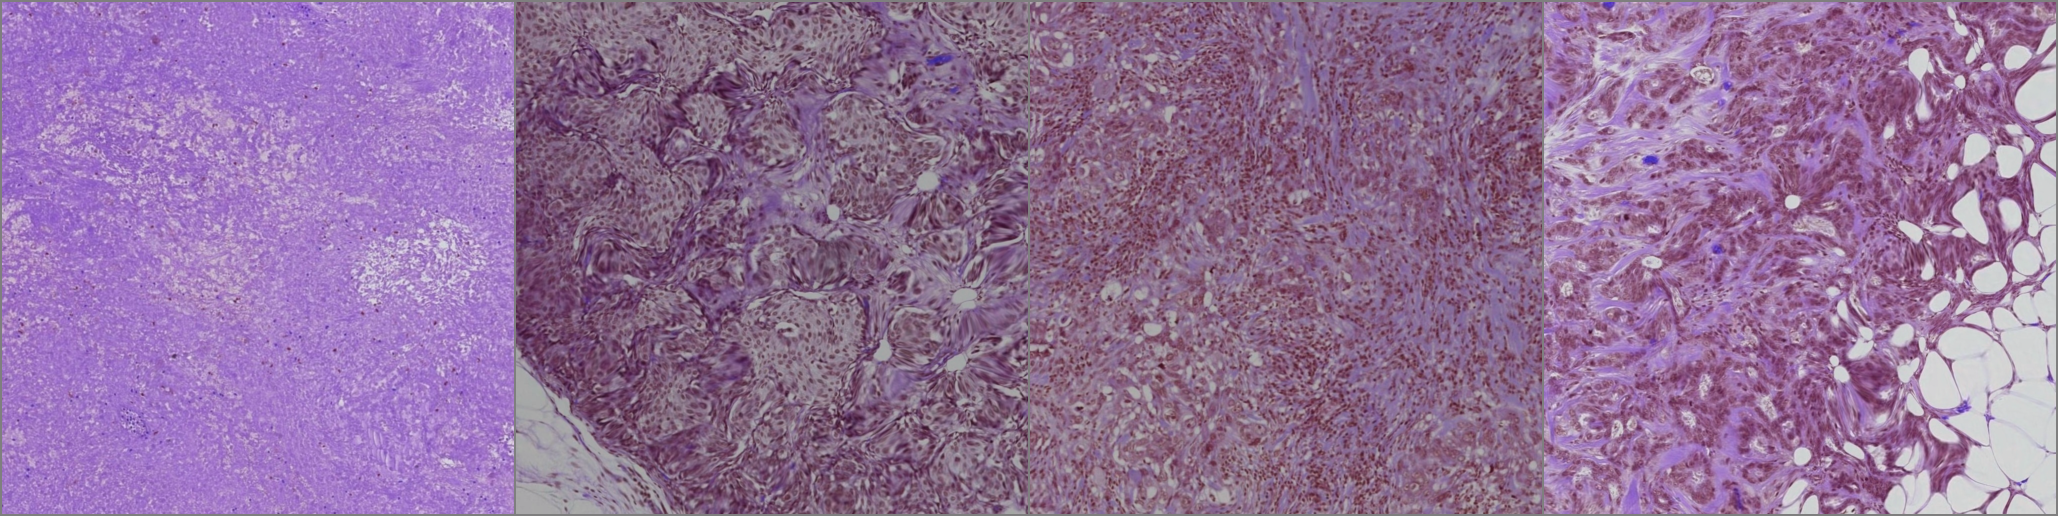
\includegraphics[width=1\linewidth]{5_Results/figures/control_gs-020380_e-000020_b-000900.png}
    \caption[Input H\&E images for train log at e=20, steps=900]{H\&E Stain - Input}
    \label{fig:train-log-source-e20-s900}
\end{figure}
\begin{figure}[h]
    \centering
    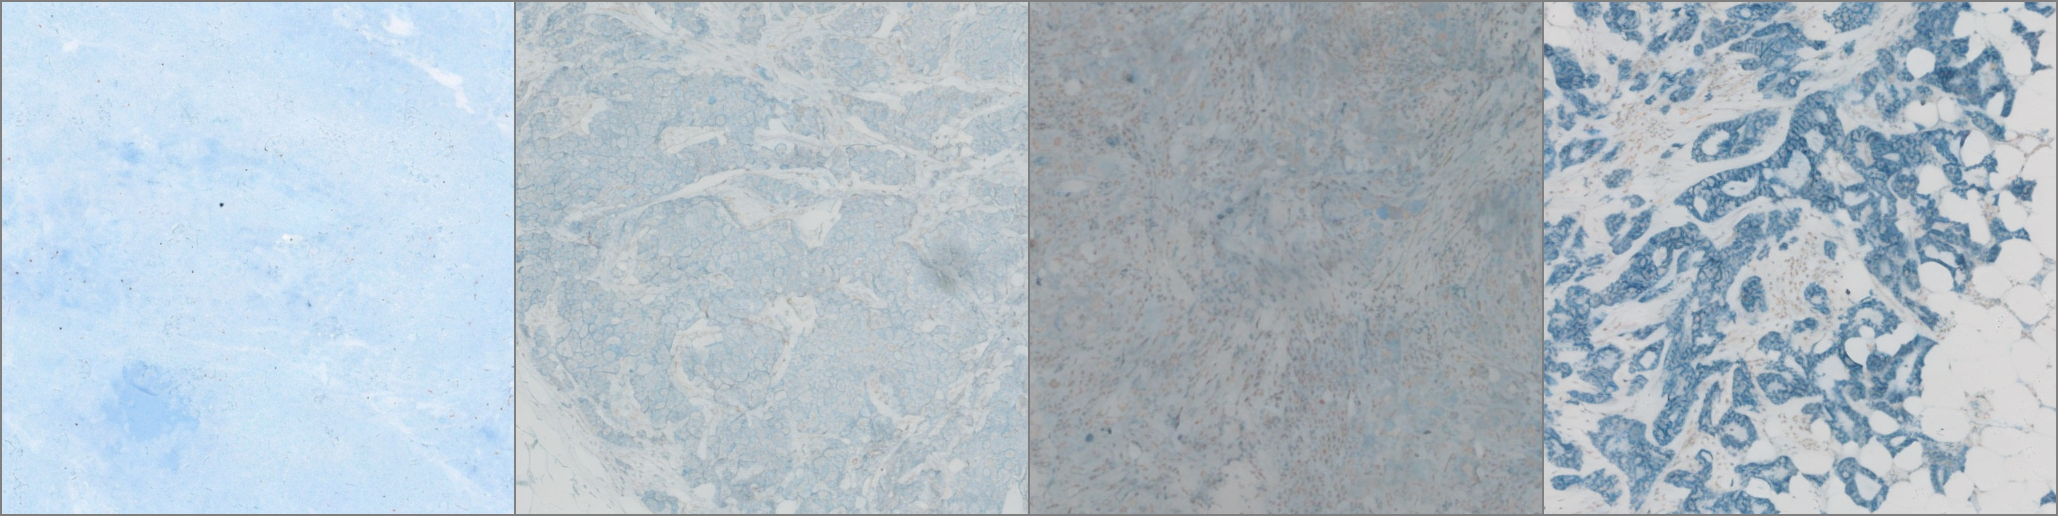
\includegraphics[width=1\linewidth]{5_Results/figures/reconstruction_gs-020380_e-000020_b-000900.png}
    \caption[Target IHC images for train log at e=20, steps=900]{IHC Stain - Ground Truth}
    \label{fig:train-log-target-e20-s900}
\end{figure}
\begin{figure}[h]
    \centering
    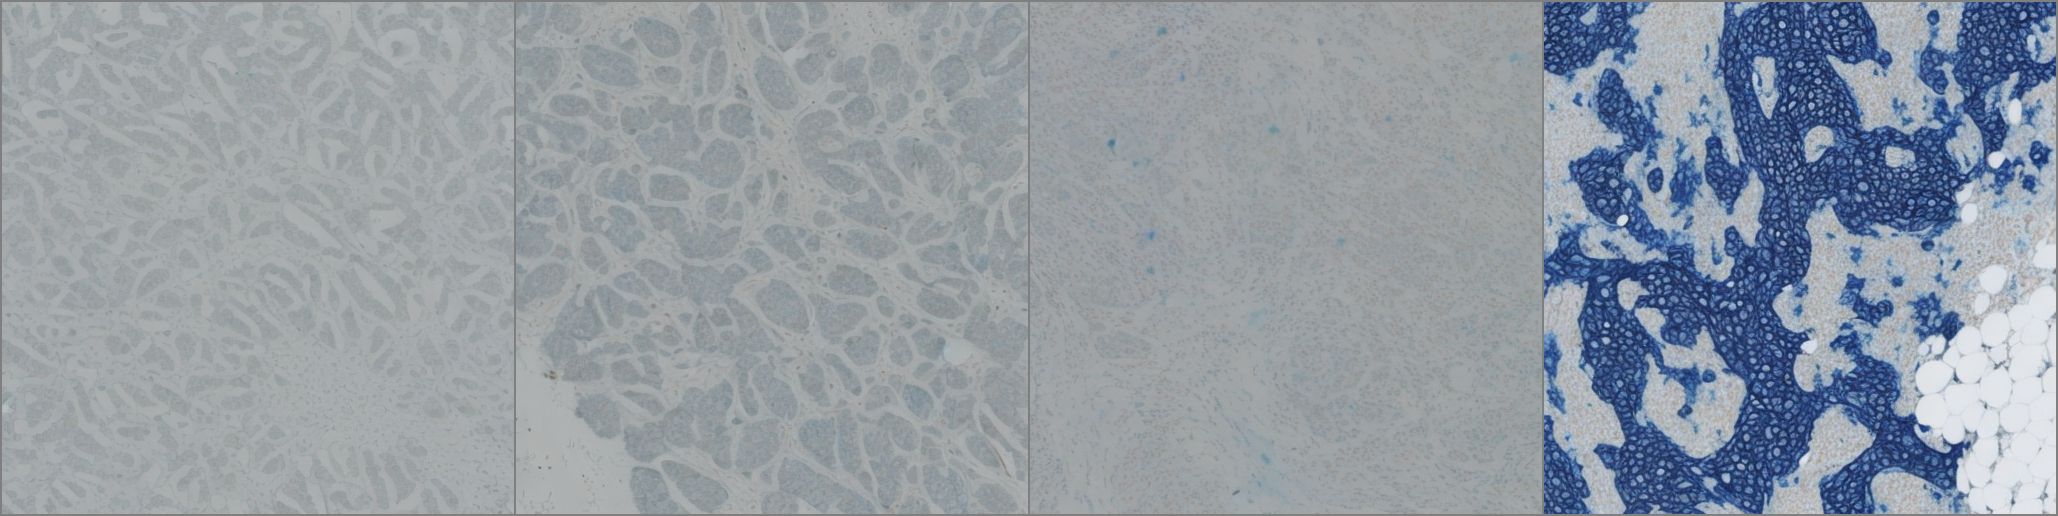
\includegraphics[width=1\linewidth]{5_Results/figures/samples_cfg_scale_9.00_gs-020380_e-000020_b-000900.png}
    \caption[Generated IHC images for train log at e=20, steps=900]{IHC Stain - Generated}
    \label{fig:train-log-sample-e20-s900}
\end{figure}
\begin{figure}[h]
    \centering
    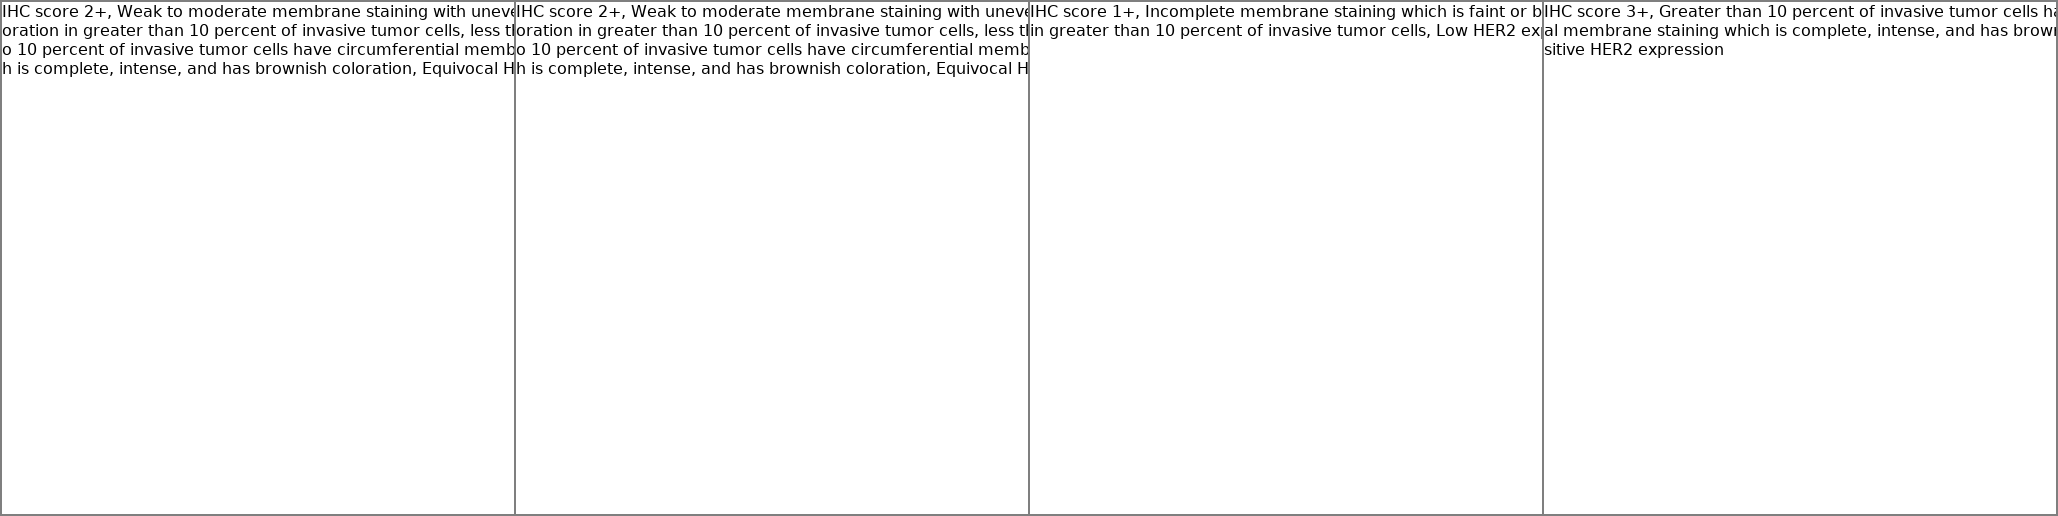
\includegraphics[width=1\linewidth]{5_Results/figures/conditioning_gs-020380_e-000020_b-000900.png}
    \caption[Input prompts for train log at e=20, steps=900]{IHC Score + Prompt. IHC scores from left to right are 2+. 2+. 1+ and 3+}
    \label{fig:train-log-prompt-e20-s900}
\end{figure}

\subsection{Model variation 1: SD Unlocked}

From the loss metrics of Figures \ref{fig:mod2-train-loss-epoch} and \ref{fig:mod2-train-loss-epoch-smooth}, there is a lot more variability here between epochs. The smoothed graph also suggests a plateaued trend line. But, from the loss curve, we can see that the penultimate epoch of 49 achieved a loss of 0.1756 which is slightly lower than the least value from model 1. This seems to suggest that training the SD layers along with the copy has the potential for better fitting with the objective but the number of epochs might again be too low to make any definitive conclusion.
\begin{figure}[h]
    \centering
    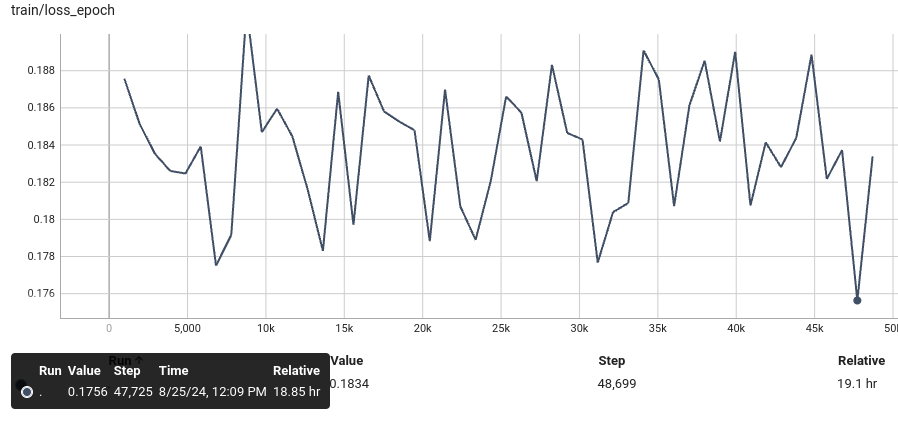
\includegraphics[width=1\linewidth]{5_Results/figures/sd2-train-loss-epoch.png}
    \caption{Model 2: Train loss/epoch}
    \label{fig:mod2-train-loss-epoch}
\end{figure}

\begin{figure}[h]
    \centering
    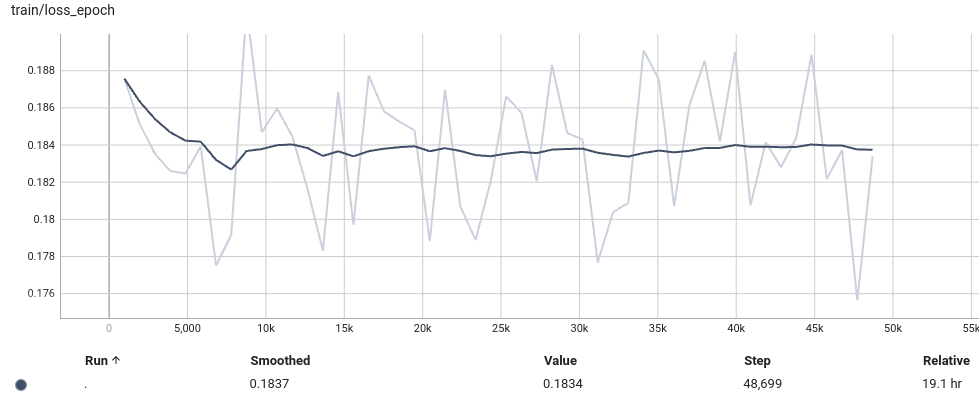
\includegraphics[width=1\linewidth]{5_Results/figures/model-2-train-epoch-loss-smooth.png}
    \caption{Model 2: Train loss/epoch with smoothing=0.9}
    \label{fig:mod2-train-loss-epoch-smooth}
\end{figure}

\section{Objective Evaluation}

As discussed in section 3.3.2, objective evaluation of the test results is not ideal to gauge the effectiveness of the trained model. The results are tabulated in Table \ref{tab:obj-results}.

\begin{table}[H]
\begin{center}
\begin{tabular}{|>{\raggedright\arraybackslash}p{0.3\linewidth}|>{\raggedright\arraybackslash}p{0.35\linewidth}|>{\raggedright\arraybackslash}p{0.35\linewidth}|}
\hline 
\textbf{Model}& \textbf{PSNR(dB)}& \textbf{SSIM}\\ \hline 
CycleGAN& 16.203& 0.373\\ \hline
pix2pix(unet generator)& 18.654& 0.419\\ \hline
Pyramid pix2pix& \textbf{21.160}& \textbf{0.477}\\ \hline
SD Locked (with prompt)& 14.54& 0.3808\\ \hline
SD Locked (without prompt)& 11.86& 0.3084\\ \hline
\end{tabular}
\caption[PSNR and SSIM metrics for the models discussed]{PSNR and SSIM metrics for the models discussed. Note that the CycleGAN and two pix2pix implementation metrics have been taken from \textcite{Liu2022BCI:Pix2pix}[Table 1, p. 7]}\label{tab:obj-results}
\end{center}
\end{table}

From these metrics, the Pyramid pix2pix model is still the one to beat by a long shot compared to our models. The only gain than any other model is in the SSIM category against CycleGAN which is already relatively obsolute for this field. Also, as expected, the model tested with the prompt is the better performing model with a 0.08 point lead compared to the test without prompts ad isn't too bad compared to pix2pix(unet). This gives hope that considering for how little time it was trained, there and the loss trend, there is alot of growth for improvement with just more training and experimentation with hyper-parameters like learning rate.

\section{Subjective Validation}

\begin{figure}[h]
    \centering
    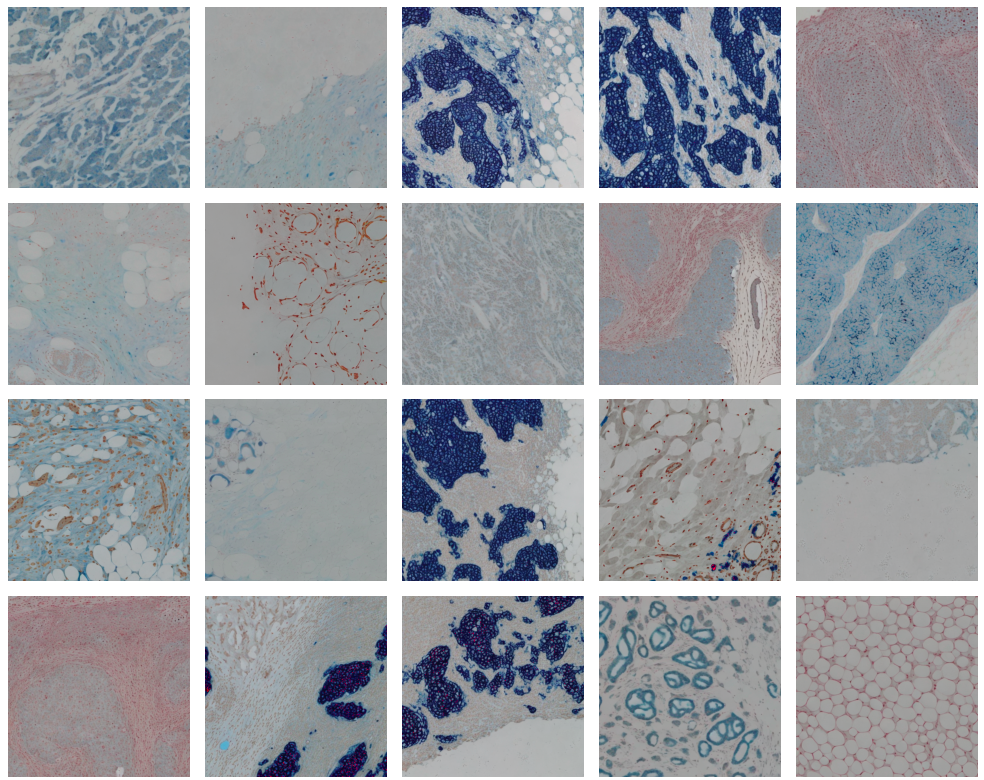
\includegraphics[width=1\linewidth]{5_Results/figures/subjective-eval-samples.png}
    \caption{A grid of 20 randomly selected generated IHC image patches for subjective validation}
    \label{fig:sub-eval-grid}
\end{figure}

For the subjective validation of manual scoring of 20 random generated IHC images the accuracy turned out to be on par with the highest accuracy obtained by two independent pathologists in the case of \textcite{Liu2022BCI:Pix2pix}[Table 5, p. 8] which \textbf{40\%}. Now, this is not an extensive sample size and in the paper they selected 40 images instead of 20. But again, as we've seen in previous examples, there is a lot of potential.

\begin{figure}[h]
    \centering
    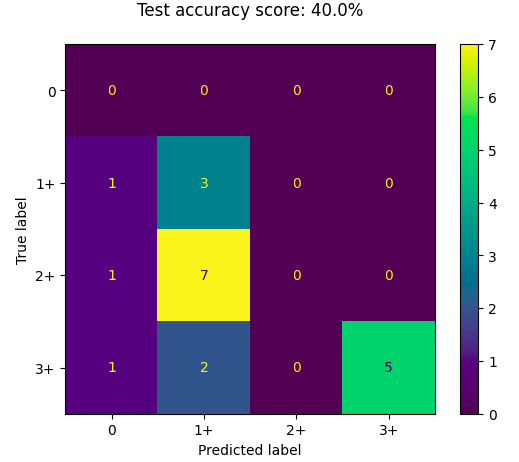
\includegraphics[width=1\linewidth]{5_Results/figures/subj-eval-confusion-matrix.png}
    \caption{Confusion matrix report of subjective validation resilts}
    \label{fig:conf-mat}
\end{figure}

Figure \ref{fig:conf-mat} shows the various accuracies across the four classes with 3+ performing the best understandably because these images have the most distinguishable morphological features standing out from the IHC stain. 2+ had a zero percent accuracy with it being mistaken for the 1+ class over 7 times by the model. There are also no successful class 0 predictions and the lack of candidates in the sample size again points out the data imbalance issue with the dataset.

\section{Key Limitations}

The biggest limitation with the research performed in this thesis is that the trained model is purely generative and does not have the capabilities to act as a classifier which is what we would want and was part of the original research goals. It just ended out to be out of the scope for this master's thesis on account of time and resource constraints. Thus in its current state, the trained model does not pose any real world application and is best to be considered a proof-of-concept of Stable Diffusion's capability in conjunction with ControlNet. 

The second key limitation in the methodology of this research is the lack of variable experimentation with different hyper-parameters which would have potentially yielded better results.

% ---------------------------------------------------------------------------
%: ----------------------- end of thesis sub-document ------------------------
% ---------------------------------------------------------------------------

